\part{Analyse de l'existant}


\section{Fonctionnement de l'application Royal}

Comme nous pouvons l'observer le MCD existant n'est pas parfaitement obtimisé et certaines des informations ne sont jamais utilisé dans l'aplication Royal. 

\subsection{Introduction}
Nous n'avions pas d'existant imposé à proprement parlé, cependant nous avons été guidé vers Royal, un projet existant réalisé par des étudiants du département informatique l'an passé.
Il apparait être une des solutions actuelles la plus en accord avec la demande client à savoir de manière générale, « la facilitation de gestion d'une bédéthèque ».

De ce fait, cet article traitera du fonctionnement de Royal.
Royal est une application 
libre \footnote{Selon les termes de la GNU Lesser General Public License}
issus d'une amélioration de Birdy, une autre application libre de gestion de livre.

\subsection{Aspect fonctionnel de Royal}
Royal permet la saisie d'informations sur une bande déssinée (BD), tel que son titre, son auteur, son image de couverture (recherchée sur internet), sa date de parution, etc..
Il permet d'obtenir une liste de l'ensemble des BDs, que l'on peut trier selon divers critères et réorganiser selon des collections de BDs.
Royal permet l'enregistrement de BDs, mais aussi d'informations concernant les auteurs ou encore les collections.
L'on peut aussi importer un ensemble de BD à partir d'une base de donnée existante.
De plus Royal intègre un système multilangue concernant son interface utilisateur, ainsi que d'une bibliothèque d'aide d'utilisation.

\subsection{Aspect technique de Royal}
Royal est développé en Java et utilise la bibliothèque \emph{Swing} pour son environnement graphique. 
Le projet à été développé sous Linux, mais reste néanmoins éxécutable sous d'autres systèmes d'exploitations comme Windows 7 par exemple, avec plus ou moins de succès. 
L'ensemble des données stockées est fait via \emph{Hibernate}, c'est un framework gérant la persitance des objets en base de données. 
C'est un outil lourd et complexe mais très puissant que nous allons réutiliser étant donné sa mise en place existante sous Royal qui permet un transfert simplifié entre objets java et base de données.

\subsection{Analyse de la base de données déjà existante}
\begin{figure}[h]
\begin{center}
 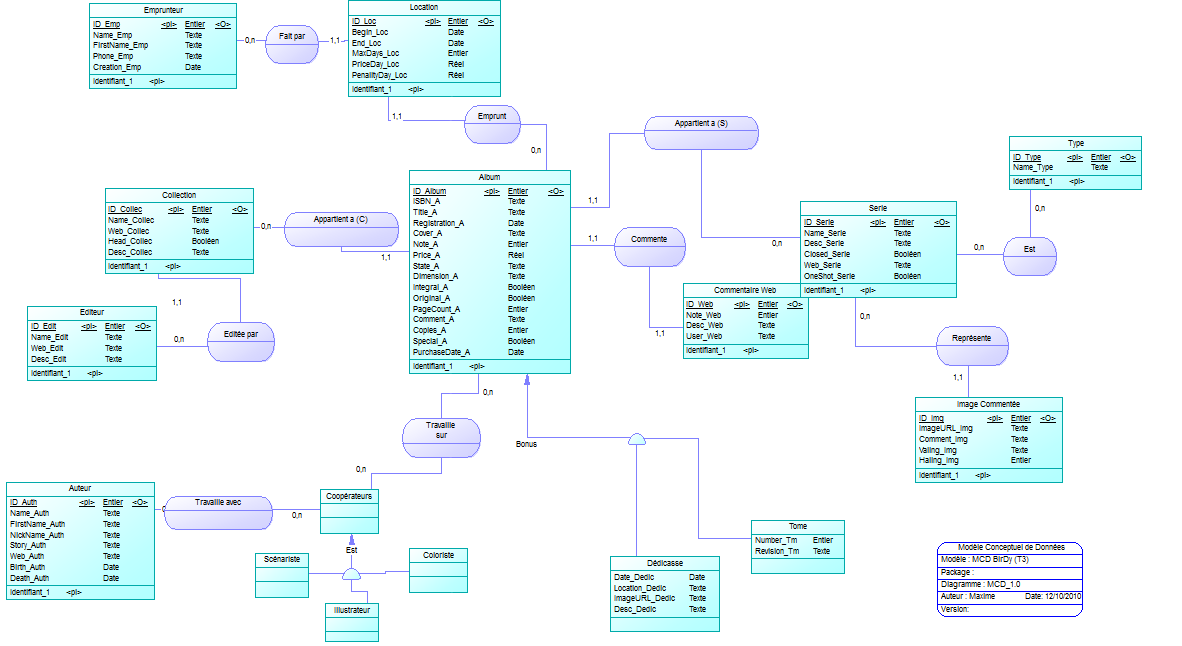
\includegraphics[height=6cm]{../img/MCD_Royal.png}
\end{center}
\caption{MCD Repris de la documentation déjà existante de Royal}
\end{figure}
